\documentclass[9pt]{beamer}
\usepackage{ctex, hyperref}
\usepackage[T1]{fontenc}

% \usepackage[orientation=landscape,size=custom,width=16,height=9,scale=0.4,debug]{beamerposter}
% 修改 slides 比例,

% other packages
\usepackage{latexsym,amsmath,xcolor,multicol,booktabs,calligra}
\usepackage{graphicx,pstricks,listings,stackengine,cite}
\usepackage{subfigure}
\usepackage{tikz}
\usetikzlibrary{positioning, shapes.geometric}

\setbeamertemplate{bibliography item}[text]
\bibliographystyle{plain}
% 如果参考文献太多的话,可以像下面这样调整字体:
% \tiny\bibliographystyle{plain}

\title{多重网格大作业}
% \subtitle{毕业设计答辩}
\institute{浙江大学\ \ \ \ 数学科学学院}
\date{2024/4/10}
\usepackage{College}

% defs
\def\cmd#1{\texttt{\color{red}\footnotesize $\backslash$#1}}
\def\env#1{\texttt{\color{blue}\footnotesize #1}}
\definecolor{deepblue}{rgb}{0,0,0.5}
\definecolor{deepred}{rgb}{0.6,0,0}
\definecolor{deepgreen}{rgb}{0,0.5,0}
\definecolor{halfgray}{gray}{0.55}

\lstset{
    basicstyle=\ttfamily\small,
    keywordstyle=\bfseries\color{deepblue},
    emphstyle=\ttfamily\color{deepred},    % Custom highlighting style
    stringstyle=\color{deepgreen},
    numbers=left,
    numberstyle=\small\color{halfgray},
    rulesepcolor=\color{red!20!green!20!blue!20},
    frame=shadowbox,
}


\begin{document}

\author{黄文\hbox{\scalebox{0.6}[1]{羽}\kern-.1em\scalebox{0.5}[1]{中}}\ \ \ \ (EbolaEmperor)}

\kaishu
\begin{frame}
    \titlepage
    \begin{figure}[htpb]
        \begin{center}
            \vspace*{-0.5cm}
            
\includegraphics[width=0.2\linewidth]{pic/zju.jpg}
        \end{center}
    \end{figure}
\end{frame}

\begin{frame}
    \tableofcontents[sectionstyle=show,subsectionstyle=show/shaded/hide,subsubsectionstyle=show/shaded/hide]
\end{frame}


\section{一维情形}

\begin{frame}{V-Cycle}

\begin{figure}[H]
  \centering
  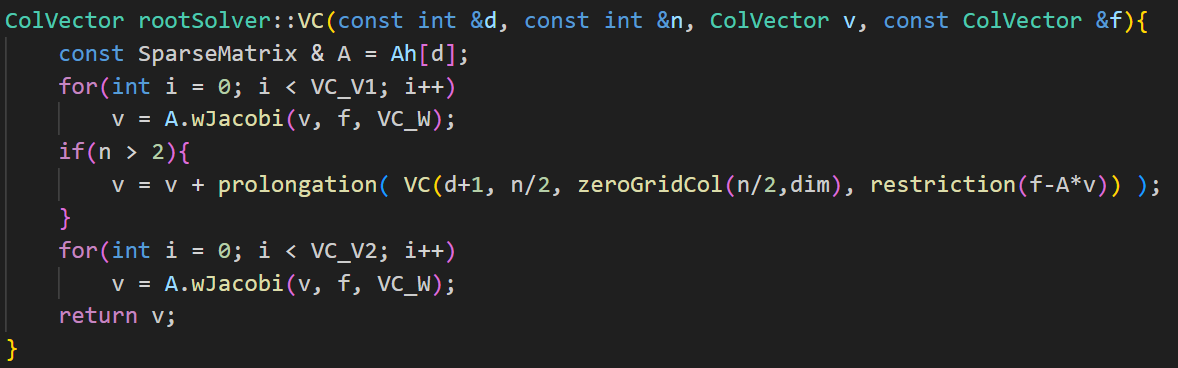
\includegraphics[width=\textwidth]{pic/v.png}
\end{figure}

\end{frame}

\begin{frame}{FMG-Cycle}

\begin{figure}[H]
  \centering
  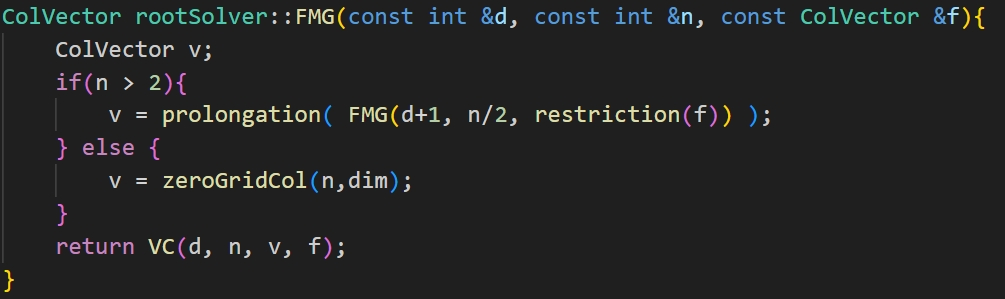
\includegraphics[width=\textwidth]{pic/FMG.png}
\end{figure}

\end{frame}

\begin{frame}{FMG的重复迭代}
理论上,一次完整的FMG就可以达到二阶精度,但是实践中,有进一步的提升空间。
\vspace{1em}\pause

假设FMG第一次迭代的结果为$\mathbf{v}$,我们可以令$\mathbf{f}'=\mathbf{f}-A\mathbf{v}$,然后将$\mathbf{f'}$作为方程右边提供给求解器,重复FMG求得$\mathbf{v}'$,此时$\mathbf{v}+\mathbf{v}'$即为两次FMG的结果。如此反复,就可以让FMG-Cycle执行多次迭代,以达到更高的求解精度。
\begin{figure}[H]
  \centering
  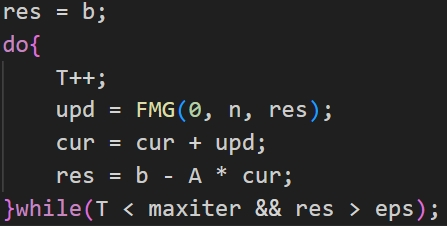
\includegraphics[width=0.4\textwidth]{pic/solve.png}
\end{figure}

\vspace{1em}\pause

在一维情形中如果使用full-weighting + 二次插值,那么一次FMG就足够达到机器精度了。二维情形则需要多次FMG以提高精度。
\end{frame}

\begin{frame}{一维情形的二次插值}
考虑用$ih,(i+1)h,(i+2)h$处的点值插值得到$ih+\frac{h}{2}$处的点值。事实上,三点唯一确定一个二次函数,直接待定系数法求出函数,再将$ih+\frac{h}{2}$代入即可,公式为:
\begin{equation}
  U^{h/2}_{2i+1} = \frac{3}{8}U^h_{i} + \frac{6}{8}U^h_{i+1} - \frac{1}{8}U^h_{i+2} + O(h^3).
\end{equation}

\pause
这样得到的公式关于$x=ih+\frac{h}{2}$不对称,为了使插值系数更加对称,我们用$(i-1)h,ih,(i+1)h$处的点值再做一次二次插值,得到:
\begin{equation}
  U^{h/2}_{2i+1} = \frac{6}{8}U^h_{i} + \frac{3}{8}U^h_{i+1} - \frac{1}{8}U^h_{i-1} + O(h^3).
\end{equation}

\pause
将上面两式相加,再乘$\frac{1}{2}$,即可得到中心对称的二次插值公式:
\begin{equation}
  U^{h/2}_{2i+1} = \frac{9}{16}U^h_{i} + \frac{9}{16}U^h_{i+1} - \frac{1}{16}U^h_{i-1} - \frac{1}{16}U^h_{i+2} + O(h^4).
\end{equation}

\pause
对于靠近边界的点,直接使用公式(3.3)会有访问越界风险,需要视点的位置使用不那么对称的(3.1)或(3.2)。
\end{frame}

\begin{frame}{一个理论问题}
用full-weighting + 二次插值效果很好,但在理论上会遇到一些问题——FMG的二阶收敛性是如何证明的?
\vspace{1em}

\pause
Lemma 9.51!它依赖于Lemma 9.50,而它又依赖于variational properties:
\begin{equation}
I_{2h}^h=c(I_h^{2h})^T,
\end{equation}
\begin{equation}
I_h^{2h}A^hI_{2h}^h=A^{2h}.
\end{equation}

上面的性质只有当$I_h^{2h}$为full-weighting算子、$I_{2h}^h$为线性插值算子时才成立!如何解决?
\vspace{1em}

\pause
An open problem.
\end{frame}

\section{二维情形}

\begin{frame}{二维情形的双线性插值}
  \small
 \begin{figure}[H]
  \centering
  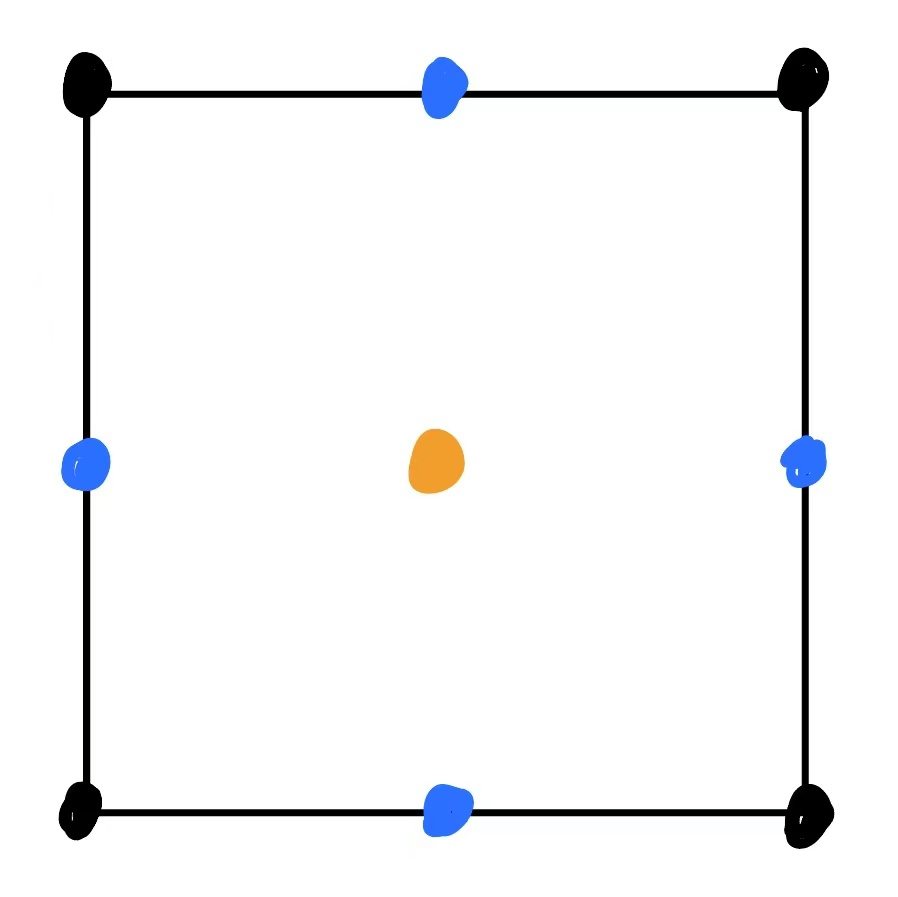
\includegraphics[width=0.3\textwidth]{pic/bilinear.jpg}
\end{figure}

\begin{itemize}
	\item 对于黑色的点,直接取粗网格点上的值;
	\item 对于蓝色的点,取粗网格上左右(或上下)两个点的平均值;
	\item 对于橙色的点,取粗网格四个角上所有点的平均值。
\end{itemize}
\end{frame}

\begin{frame}{二维情形的 “真” 线性插值}
  \small
 \begin{figure}[H]
  \centering
  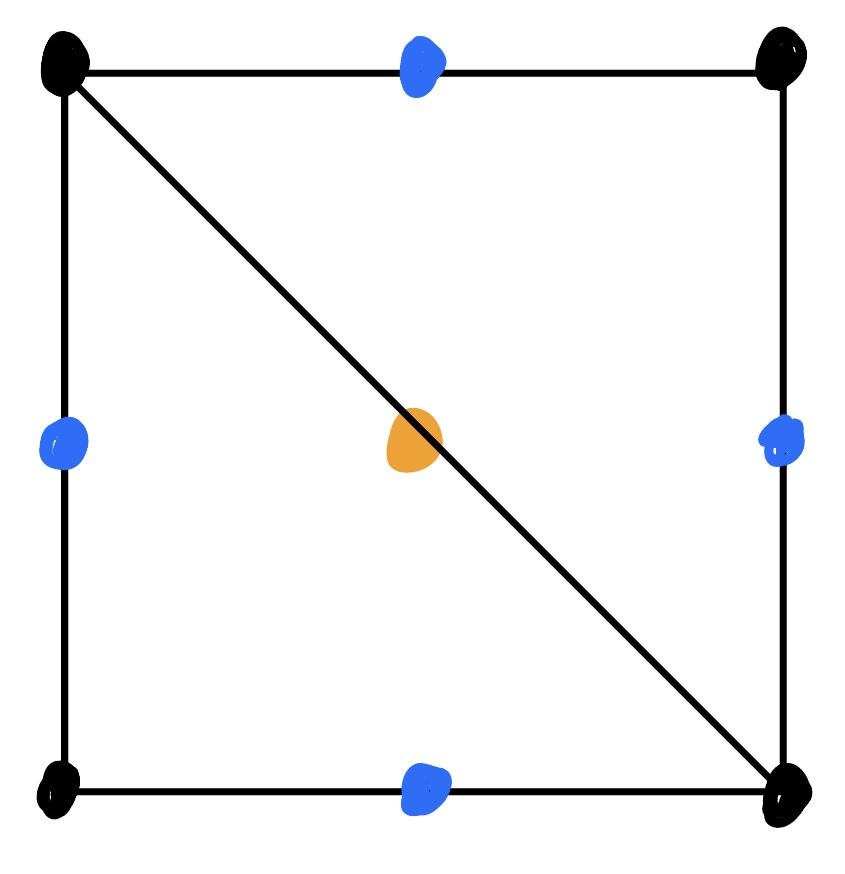
\includegraphics[width=0.3\textwidth]{pic/linear.jpg}
\end{figure}

对于每个三角形,我们可以用三角形三个顶点处的函数值拟合一个
一次函数 $p(x,y)=Ax+By+c$,
然后用这个函数计算蓝点、橙点的值。

\vspace{1em}\pause

上述做法等价于:
\begin{itemize}
	\item 对于黑色的点,直接取粗网格点上的值;
	\item 对于蓝色的点,取粗网格上左右(或上下)两个点的平均值;
	\item 对于橙色的点,取粗网格左上角、右下角两个点的平均值
\end{itemize}

事实上,这才是真正的线性插值,它和双线性插值相比,唯一的区别在于橙色的点如何计算。
\end{frame}

\begin{frame}{二维情形的二次插值}
  \small
  仍然将点分为四类。事实上,在粗网格线上的点可以使用一维的二次插值公式,唯一需要考虑的就是不在粗网格线上的点。考虑点$P_0=G^h(2i+1,2j+1)$,做一次二维二次插值需要六个点,取:
\begin{align*}
  P_1&=G^h(i,j) & P_2&=G^h(i,j+1) & P_3&=G^h(i,j+2)\\
  P_4&=G^h(i+1,j) & P_5&=G^h(i+1,j+1) & P_6&=G^h(i+1,j+2)
\end{align*}

\pause
以这六个点的点值,通过待定系数法确定一个二维二次多项式$Q(x,y)=A+Bx+Cy+Dx^2+Exy+Fy^2$,再将$P_0$代入求得点值。结果为:
\begin{equation*}
  u(P_0)=\frac{1}{2}u(P_2)-\frac{1}{8}u(P_3)+\frac{1}{2}u(P_4)+\frac{1}{4}u(P_5)-\frac{1}{8}u(P_6).
\end{equation*}

\pause
这个形式不够对称,因此我们更换$P_1,...,P_6$的选取,重复上述过程三次,将每次得到的系数在各点上相加,并乘上$\frac{1}{4}$,得到对称的二次插值公式,各点插值系数如下图所示。
\begin{figure}[H]
  \centering
  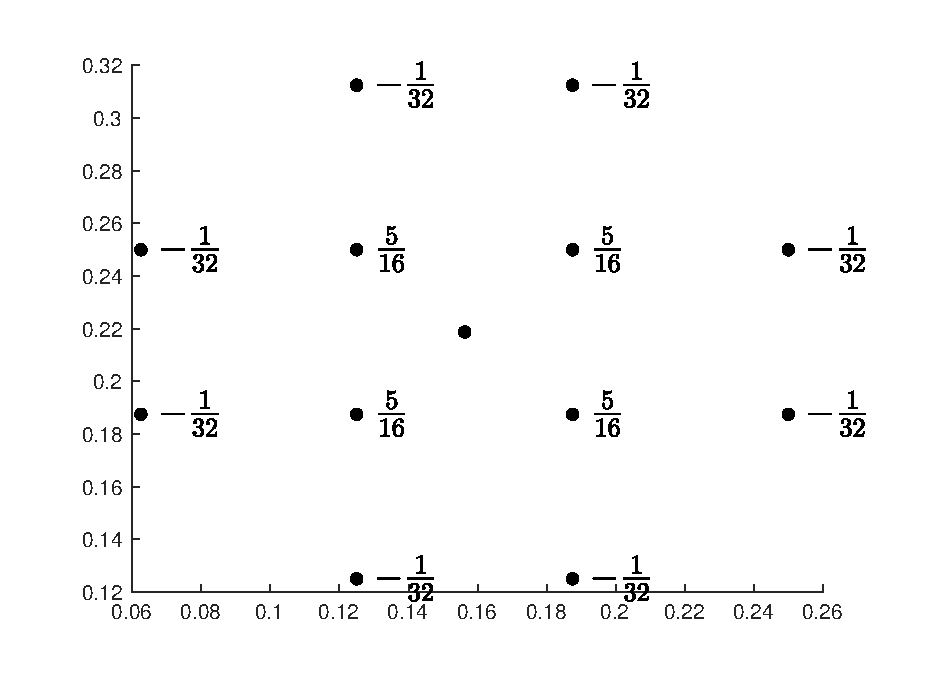
\includegraphics[width=0.4\textwidth]{../report/figure/2-1.eps}
\end{figure}

注意,上述对称的形式在边界附近会有越界问题,此时应该做特殊处理,牺牲一些对称性。
\end{frame}

\begin{frame}{与LU分解的求解速度对比}

\small
使用最佳组合full-weighting + 二次插值,与LU分解对比求解耗时(秒),结果如下。

\begin{table}[H]
  \centering
  \small
  \begin{tabular}{c|ccccccc|c}
$n$        & 16                   & 32                   & 64                   & 128                  & 256                  & 512                  & 1024                & 增长阶数 \\ \hline
V-Cycle        & 0.005 & 0.011 & 0.036 & 0.105 & 0.376 & 1.440 &  6.934 & 2.268  \\
FMG-Cycle      & 0.002 & 0.015 & 0.025 & 0.090 & 0.351 & 1.182 &  3.835 & 1.698 \\
LU分解         & 0.002 & 0.022 & 0.42 & 8.168 & - & - & - & 4.281
\end{tabular}
\end{table}

\end{frame}

\section{二维不规则情形}

\begin{frame}{方法一:切割网格}

像第一次大作业一样,把正交网格切割。

\begin{figure}[H]
  \centering
  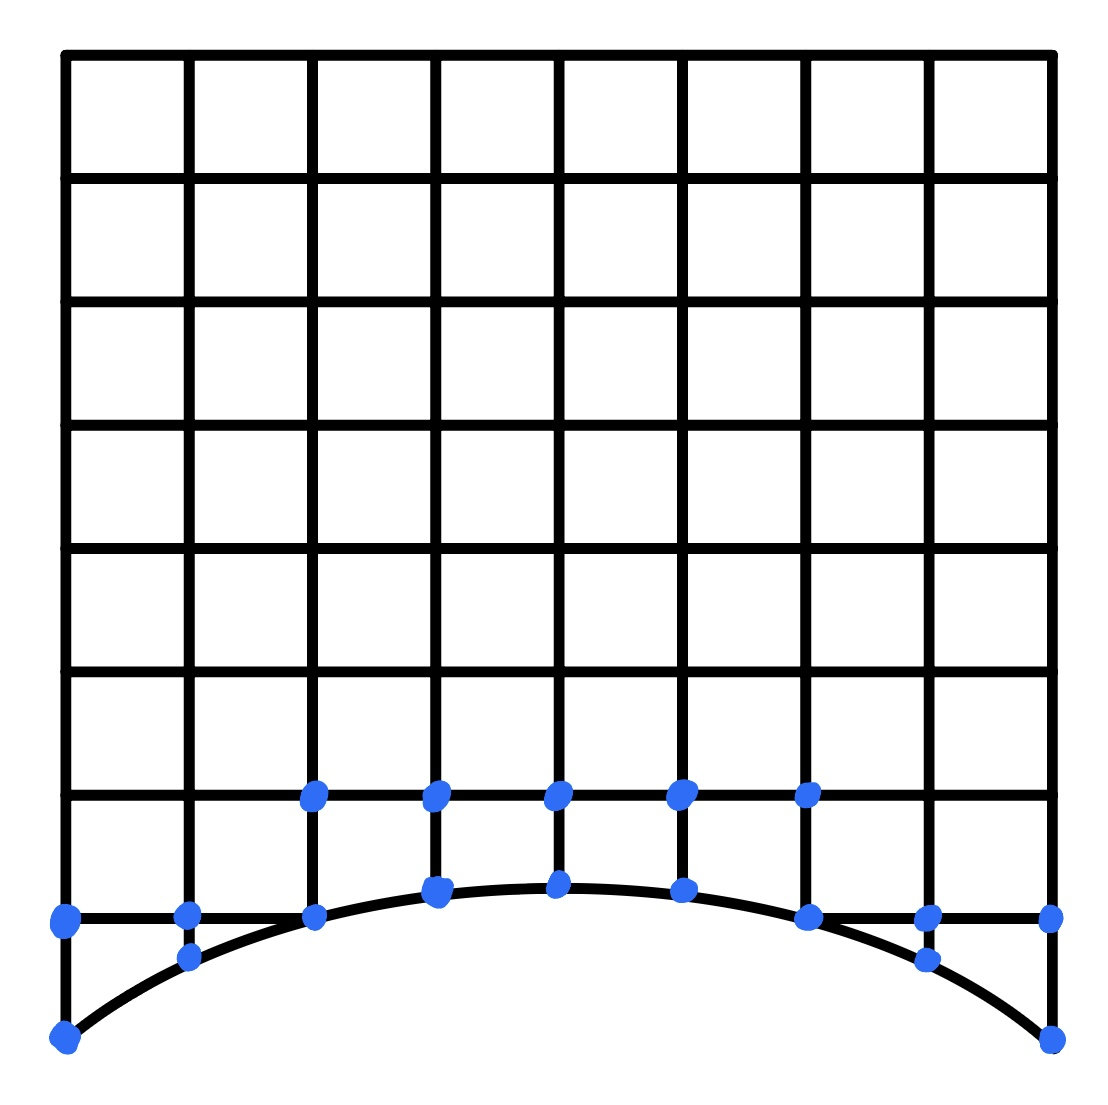
\includegraphics[width=0.3\textwidth]{pic/Irregular_CutCell.jpg}
\end{figure}

图中蓝色的点不能使用标准的 Laplace 离散格式。

\pause\vspace{1em}

因为非标准格式的存在,我们得到方程 $A\mathbf{u}=\mathbf{f}$ 之后,
如果用加权 Jacobi 迭代,会发现它不收敛。要想解决这个问题,
必须把规则格点和不规则格点分开处理,
要用到一种 “块松弛” 的技巧。

\end{frame}

\begin{frame}{方法二:区域映射}

把不规则区域映射到规则区域

\begin{figure}[H]
  \centering
  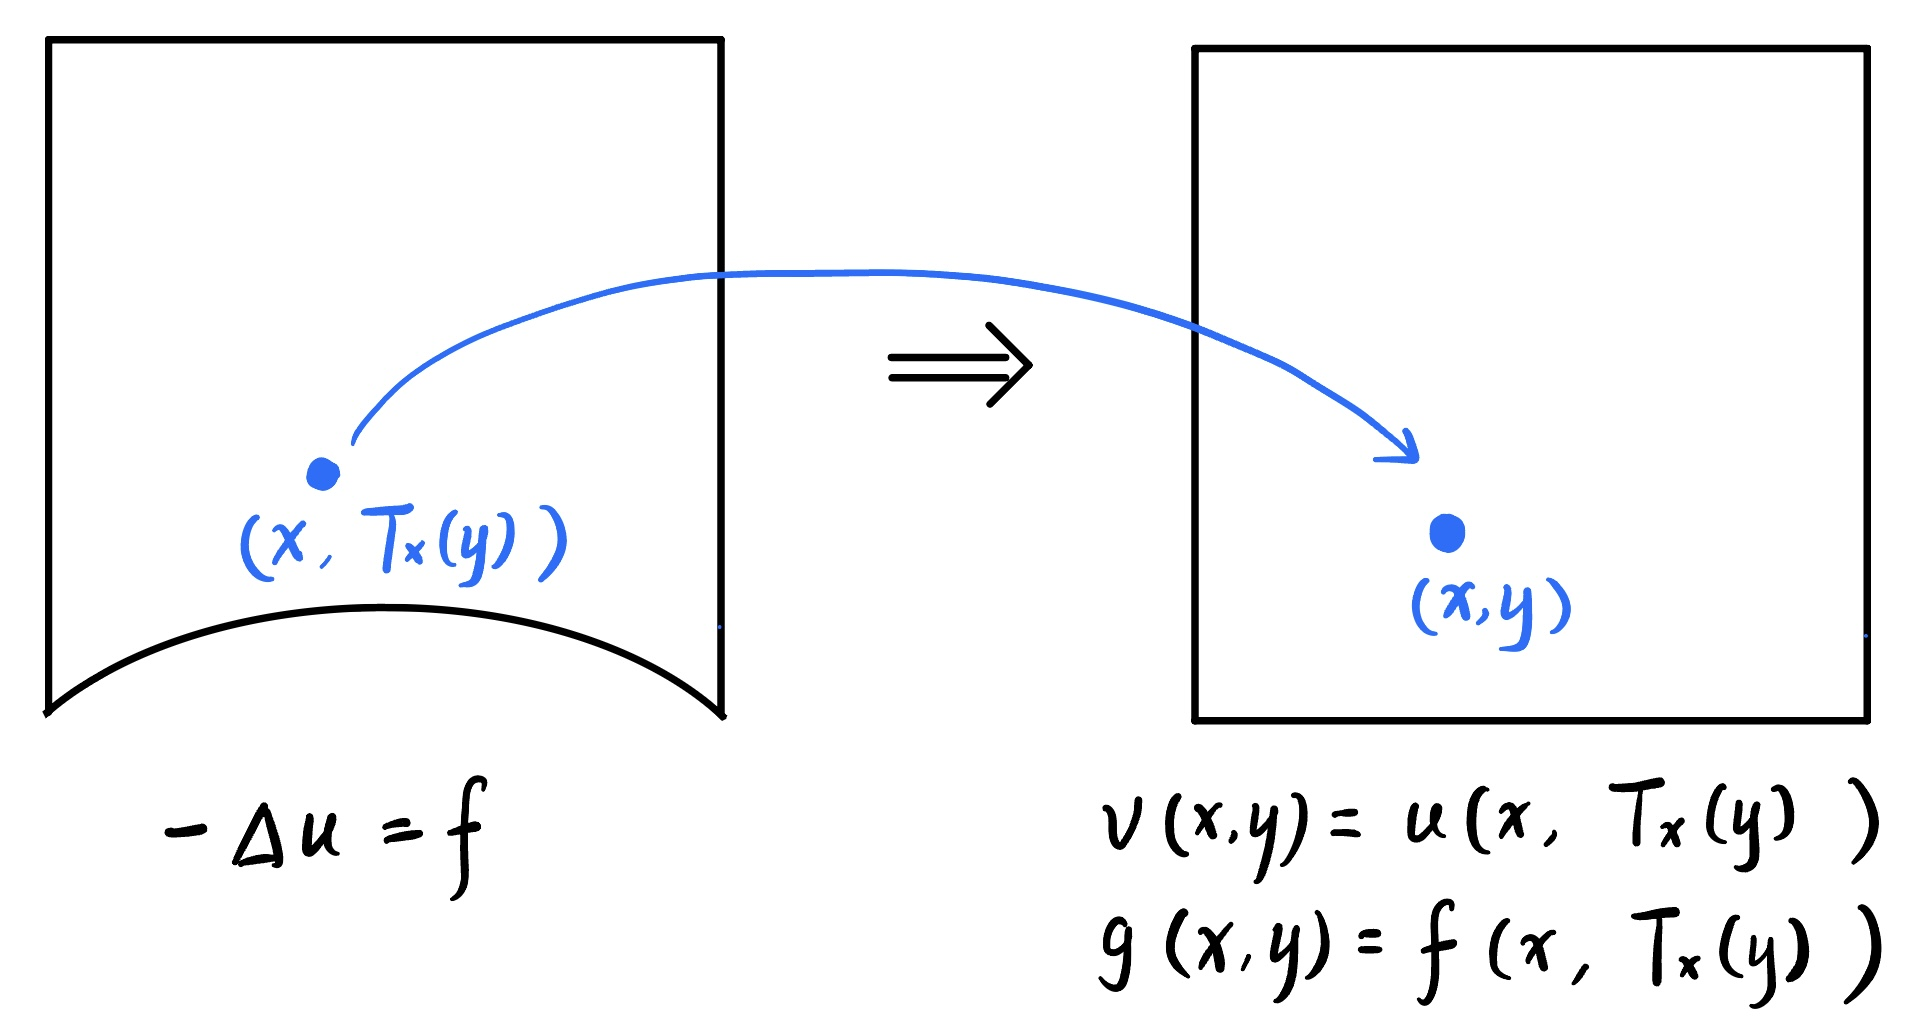
\includegraphics[width=0.6\textwidth]{pic/Irregular_Mapping.jpg}
\end{figure}

其中
\begin{equation*}
	T_x(y) = D(x) + (1-D(x))y,\quad D(x)=\frac{1}{16}\sin(\pi x).
\end{equation*}

在规则区域里求解,然后再映射回不规则区域,得到 $u$ 的数值解。

\end{frame}

\begin{frame}{方法二:区域映射}

这个方法的难点在于推导 $v$ 与 $g$ 的方程。我们有 $u(x,y)=v(x,T_x^{-1}(y))$,我们记
\begin{equation*}
	G(x,y) = T_x^{-1}(y) = \frac{y-D(x)}{1-D(x)}.
\end{equation*}
有:
\begin{equation*}
	\Delta u = v_{xx}+G_x(x,T_x(y))v_{xy}+G_y(x,T_x(y))v_{yy}+\Delta G(x,T_x(y)) v_y.
\end{equation*}
所以在规则区域中,我们要求解这样一个椭圆方程:
\begin{equation*}
	v_{xx}+G_x(x,T_x(y))v_{xy}+G_y(x,T_x(y))v_{yy}+\Delta G(x,T_x(y)) v_y = -g
\end{equation*}

\end{frame}

\begin{frame}{方法三:扭曲网格}
将整个网格沿着不规则区域的形状扭曲,如下图所示。

\begin{figure}[H]
  \centering
  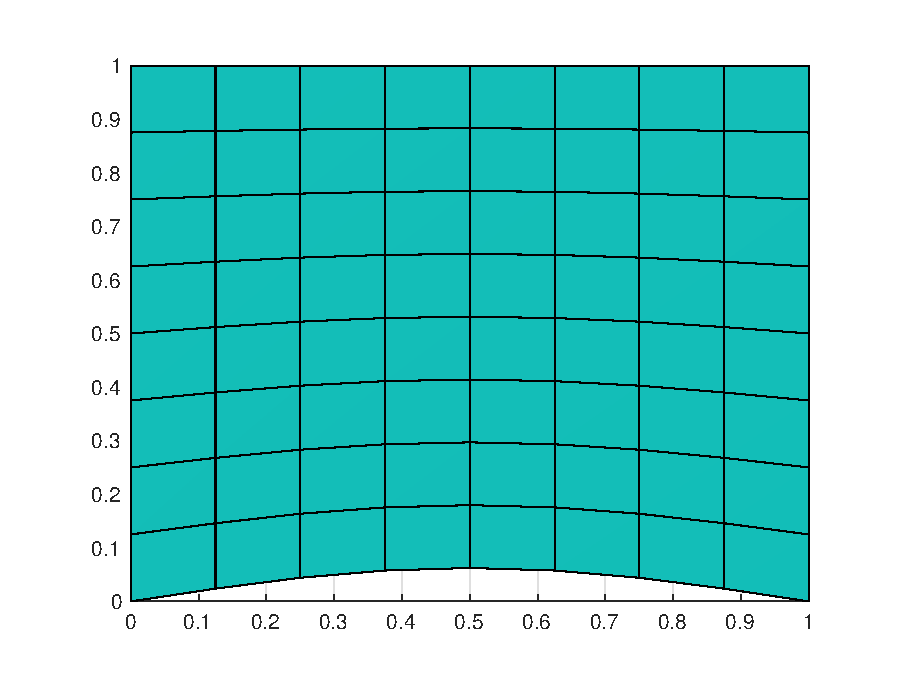
\includegraphics[width=0.5\textwidth]{../report/figure/3-1.eps}
\end{figure}

在宽度为$h=\frac{1}{n}$的扭曲网格中,网格点$G^h(i,j)$的实际坐标为:
\begin{equation}
  G^h(i,j)=(ih,\;D(ih)+jh(1-D(ih)))
\end{equation}
\begin{equation*}
D(x)=\frac{1}{16}\sin(\pi x).
\end{equation*}
\end{frame}

\begin{frame}{扭曲网格中的Laplace方程}
\small
在扭曲网格中,由于左右两个格点不在同一水平线上,因此二阶泰勒展开会存在$xy$交叉项。为将其消去,我们需要一个额外的的点。具体而言,记
\begin{align*}
  P_0&=G^h(i,j) & P_1&=G^h(i,j+1) & P_2&=G^h(i,j-1)\\
  P_3&=G^h(i+1,j) & P_4&=G^h(i-1,j) & P_5&=G^h(i+1,j+1)
\end{align*}

\pause
对于$i=0,...,5$,记$P_i=(x_i,y_i)$,将$P_i$处的点值在$P_0$处做二阶Taylor展开:
\begin{align*}
  u(P_i)&=u(P_0)+(x_i-x_0)\frac{\partial u}{\partial x}(P_0)+(y_i-y_0)\frac{\partial u}{\partial y}(P_0)
  +\frac{1}{2}(x_i-x_0)^2\frac{\partial^2 u}{\partial x^2}(P_0) \\
  & +\frac{1}{2}(y_i-y_0)^2\frac{\partial^2 u}{\partial y^2}(P_0)
  +(x_i-x_0)(y_i-y_0)\frac{\partial^2 u}{\partial x \partial y}(P_0)+O(h^3).
\end{align*}

\pause
列出六元一次方程组,解出系数$A_0,...,A_6$,使得
\begin{equation*}
  \sum_{i=0}^6 A_iu(P_i)=-\Delta u(P_0)+O(h)
\end{equation*}

\pause
这样列出的方程不够美观。因此我们更换$P_5$的选取,分别选择$G^h(i+1,j-1),G^h(i-1,j+1),G^h(i-1,j-1)$重复上述过程,一共求得四组系数,将各组系数在对应点处相加,再乘以$\frac{1}{4}$,即可得到更加对称的离散化Laplace方程。特别地,在靠近边界的格点处,上述过程会存在越界风险,因此需要视格点位置做特殊处理。
\end{frame}

\begin{frame}{扭曲网格中的Laplace方程}
以$n=32,i=4,j=6$为例,通过上述方法求得的各点系数如下图所示,可以看到大体上与规则网格类似。

\begin{figure}[H]
  \centering
  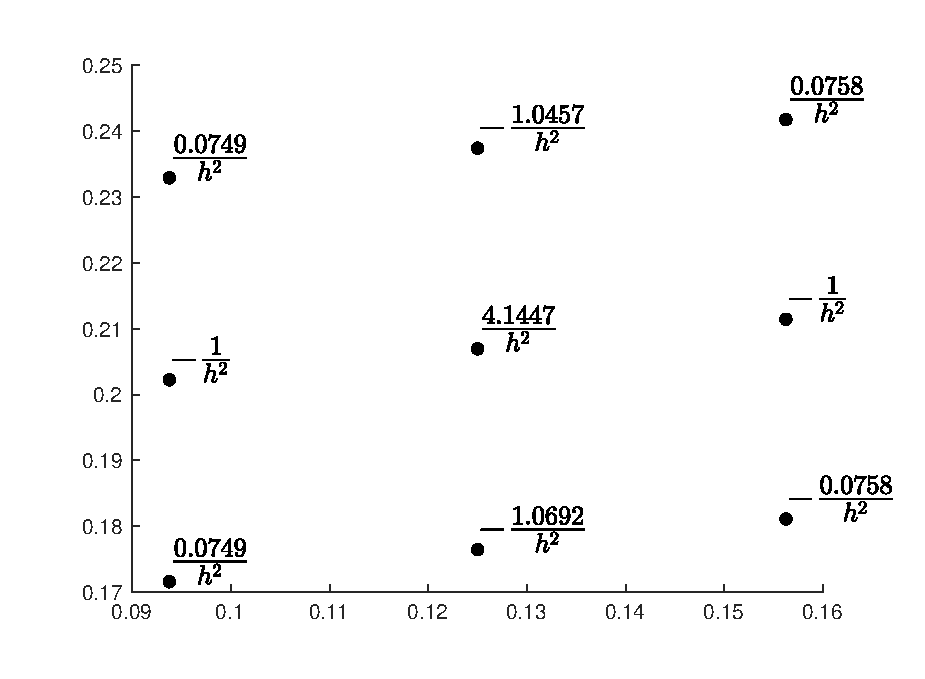
\includegraphics[width=0.5\textwidth]{../report/figure/3-2.eps}
\end{figure}
\end{frame}

\begin{frame}{扭曲网格中的Neumann边界条件}
\small
这里仅以$x=0$边界为例,其它边界的想法时类似的。在扭曲网格中,$U_{0,j},U_{1,j},U_{2,j}$这三点之间存在$y$方向的偏移,因此二阶Taylor展式中存在$y,y^2,xy$项,这就需要额外的三个点来消除。与Laplace方程的方法完全类似,选取六个点:
\begin{align*}
  P_0&=G^h(0,j) & P_1&=G^h(1,j) & P_2&=G^h(2,j)\\
  P_3&=G^h(0,j-1) & P_4&=G^h(0,j+1) & P_5&=G^h(1,j+1).
\end{align*}

\pause
对于$i=0,...,5$,我们记$P_i=(x_i,y_i)$,将$P_i$处的点值在$P_0$处做二阶Taylor展开:
\begin{align*}
  u(P_i)&=u(P_0)+(x_i-x_0)\frac{\partial u}{\partial x}(P_0)+(y_i-y_0)\frac{\partial u}{\partial y}(P_0)
  +\frac{1}{2}(x_i-x_0)^2\frac{\partial^2 u}{\partial x^2}(P_0) \\
  & +\frac{1}{2}(y_i-y_0)^2\frac{\partial^2 u}{\partial y^2}(P_0)
  +(x_i-x_0)(y_i-y_0)\frac{\partial^2 u}{\partial x \partial y}(P_0)+O(h^3).
\end{align*}

\pause
列出六元一次方程组,解出系数$A_0,...,A_6$,使得
\begin{equation*}
  \sum_{i=0}^6 A_iu(P_i)=-u_x(P_0)+O(h^2)
\end{equation*}

为使方程更加对称,我们更换$P_5$的选取,取$P_5=G^h(1,j-1)$,重复上述过程,得到另一组系数,将各组系数在对应点处相加,再乘以$\frac{1}{2}$,即可得到更加对称的Neumann边界条件方程。特别地,在靠近上下边界的格点处,上述过程会存在越界风险,因此需要视格点位置做特殊处理。
\end{frame}

\begin{frame}{扭曲网格中的Neumann边界条件}
以$n=32,j=6$为例,通过上述方法求得的各点系数如下图所示,可以看到大体上与规则网格类似。

\begin{figure}[H]
  \centering
  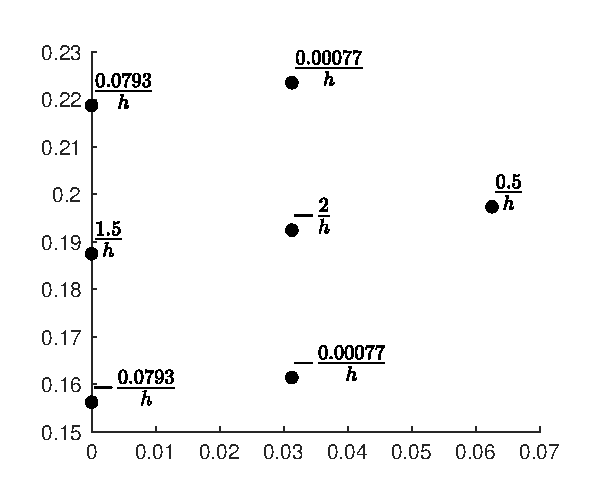
\includegraphics[width=0.5\textwidth]{../report/figure/3-3.eps}
\end{figure}
\end{frame}

\begin{frame}{扭曲网格中的线性插值}
\small
对于一个细网格上的点,它的位置可能有四种情况:在粗网格点上、在粗网格的某条竖直线上、在粗网格的某条水平线上、不在粗网格线上。对于前两种情况,我们的处理方式与规则网格一样。对于第三种情况,因为扭曲网格的格点与左右两格点并不在同一直线上,因此需要引入第三点做线性插值。

\pause
我们只介绍不在粗网格线上点如何插值。考虑点$P_0=G^h(2i+1,2j+1)$,选取粗网格上三个点:
\begin{align*}
  P_1&=G^{2h}(i,j) & P_1&=G^{2h}(i,j+1) & P_2&=G^{2h}(i+1,j)
\end{align*}

\pause
对于$i=0,...,3$,我们记$P_i=(x_i,y_i)$,将$P_i$处的点值在$P_0$处做一阶Taylor展开:
\begin{align*}
  u(P_i)&=u(P_0)+(x_i-x_0)\frac{\partial u}{\partial x}(P_0)+(y_i-y_0)\frac{\partial u}{\partial y}(P_0)
  +\frac{1}{2}(x_i-x_0)^2\frac{\partial^2 u}{\partial x^2}(P_0) + O(h^2).
\end{align*}

\pause
列出三元一次方程组,解出系数$A_1,...,A_3$,使得
\begin{equation*}
  \sum_{i=1}^3 A_iu(P_i)=u(P_0)+O(h^2)
\end{equation*}

为了使插值系数更加对称,我们重新选取$P_1,P_2,P_3$,每次在$P_0$周围的四个粗网格点上取三个点做上述过程,取遍所有可能,一共四次。将每次得到的系数在各点处相加并乘$\frac{1}{4}$,即可得到更加对称的线性插值方程。
\end{frame}

\begin{frame}{扭曲网格中的线性插值}
以$n=32,i=5,j=7$为例,各点插值系数如下图所示,与规则网格的插值系数只相差大约$0.001$.
\begin{figure}[H]
  \centering
  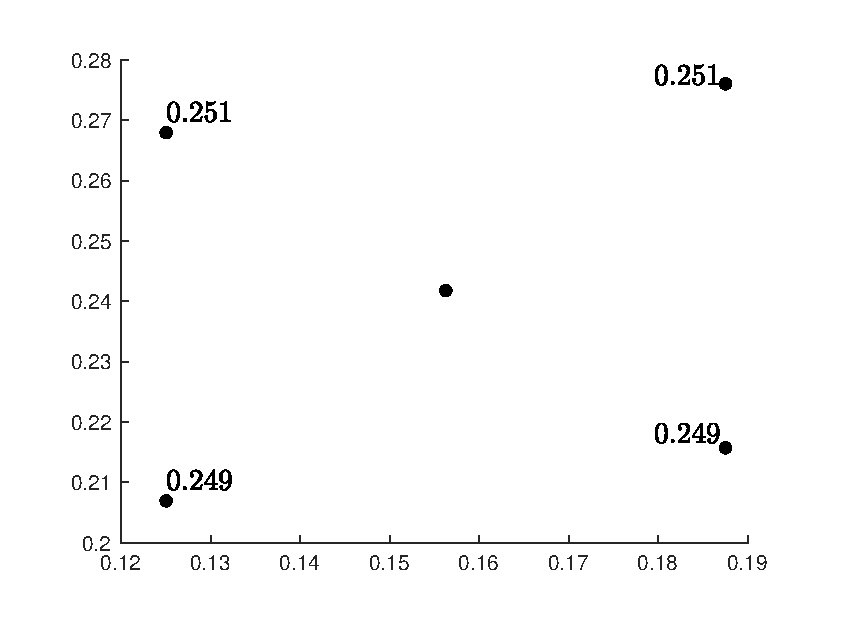
\includegraphics[width=0.5\textwidth]{../report/figure/3-5.eps}
\end{figure}

\pause
在最早先版本的代码中,我们实现了不规则网格的线性插值,当时我们并没有发现插值系数与规则网格如此相近。意识到这个情况后,在最终版本的代码中,出于计算性能考虑,我们选择直接使用规则网格的线性插值作为近似。

\pause
\vspace{1em}
二次插值思路类似:Taylor展开后求系数、对称化,不再赘述。
\end{frame}

\begin{frame}{扭曲网格的效果}
\small
考虑由精确解$u(x,y)=e^{\sin x+y}$导出的Dirichlet边值问题,用$n=16,32,64,128,256,512,1024$的网格测试,使用V-Cycle,限制算子选择Full Operator,插值算子选择线性插值。当$n=16,32,64,128$时,误差分布如下图所示。
\begin{figure}[H]
  \centering
  \tiny
  \begin{minipage}[t]{0.24\linewidth}
      \centering
      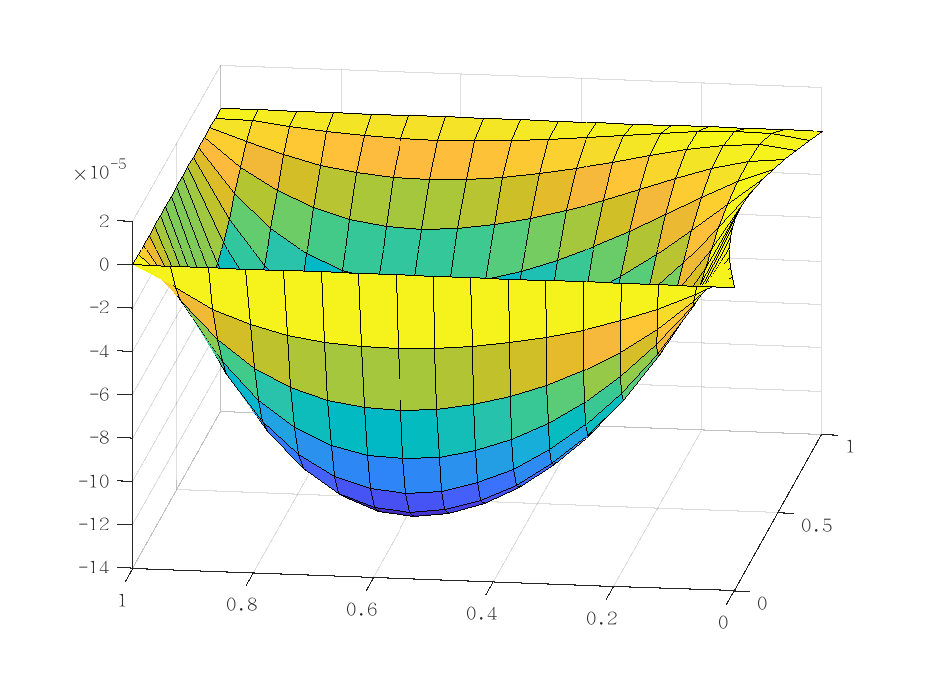
\includegraphics[width=0.95\linewidth]{../report/figure/3-1-1.eps}
  \end{minipage}
  \begin{minipage}[t]{0.24\linewidth}
    \centering
    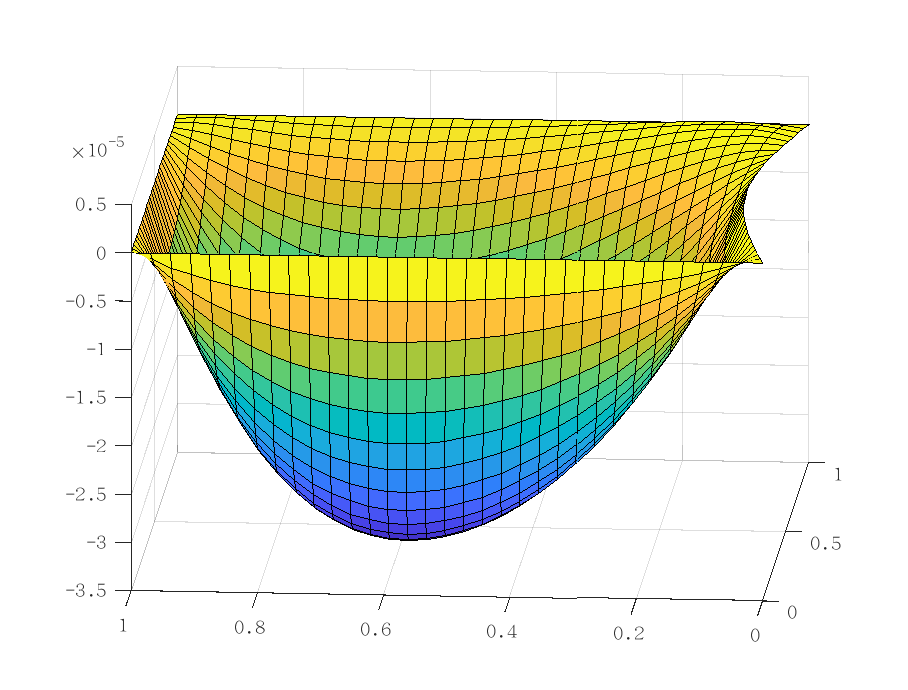
\includegraphics[width=0.95\linewidth]{../report/figure/3-1-2.eps}
  \end{minipage}
  \begin{minipage}[t]{0.24\linewidth}
    \centering
    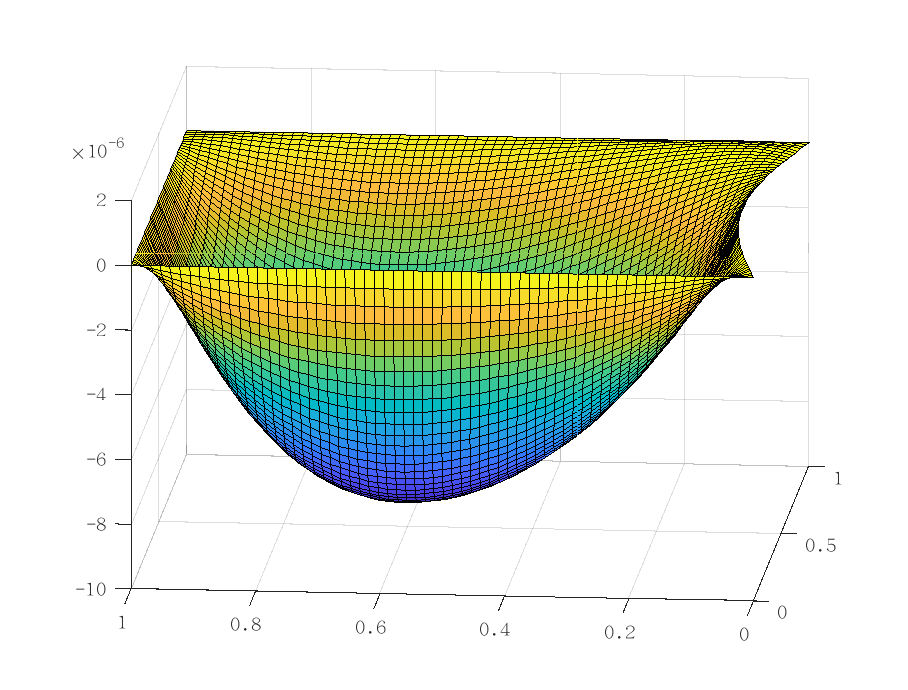
\includegraphics[width=0.95\linewidth]{../report/figure/3-1-3.eps}
  \end{minipage}
  \begin{minipage}[t]{0.24\linewidth}
    \centering
    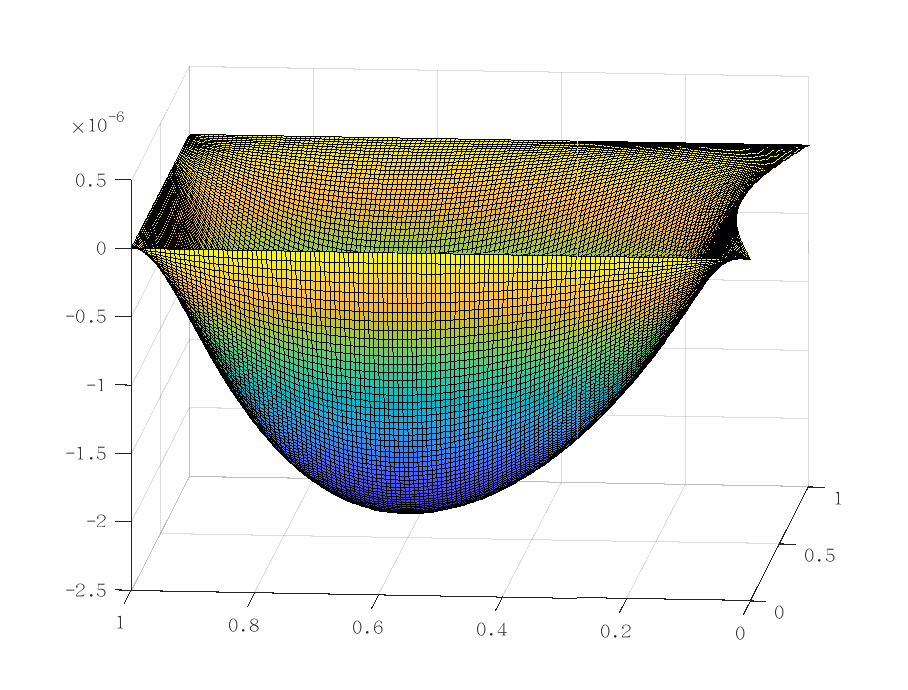
\includegraphics[width=0.95\linewidth]{../report/figure/3-1-4.eps}
  \end{minipage}
\end{figure}

可以看到,在Dirichlet条件下,格点越靠近边界,最终的计算误差越小。将数值解与真实解的误差用范数估计,并根据$n=512$增加到$n=1024$时误差减小的倍数,估计各范数下的收敛阶,结果如下表。

\begin{table}
  \centering
  \tiny
  \begin{tabular}{c|ccccccc|c}
  \textbf{$n$}       & 64                   & 128                  & 256                  & 512                  & 1024                  & 收敛阶 \\ \hline
  $||\cdot||_1$      & $3.35\times 10^{-6}$ & $8.72\times 10^{-7}$ & $2.40\times 10^{-7}$ & $5.42\times 10^{-8}$ & $1.41\times 10^{-8}$ & $1.944$\\
  $||\cdot||_2$      & $4.31\times 10^{-6}$ & $1.11\times 10^{-6}$ & $2.99\times 10^{-7}$ & $6.86\times 10^{-8}$ & $1.77\times 10^{-8}$ & $1.952$\\
  $||\cdot||_\infty$ & $8.77\times 10^{-6}$ & $2.23\times 10^{-6}$ & $5.96\times 10^{-7}$ & $1.38\times 10^{-7}$ & $3.54\times 10^{-8}$ & $1.958$
  \end{tabular}
\end{table}

大致呈二阶收敛。
\end{frame}

\section{程序设计}

\begin{frame}{参数管理}
\small
\begin{figure}[H]
\centering
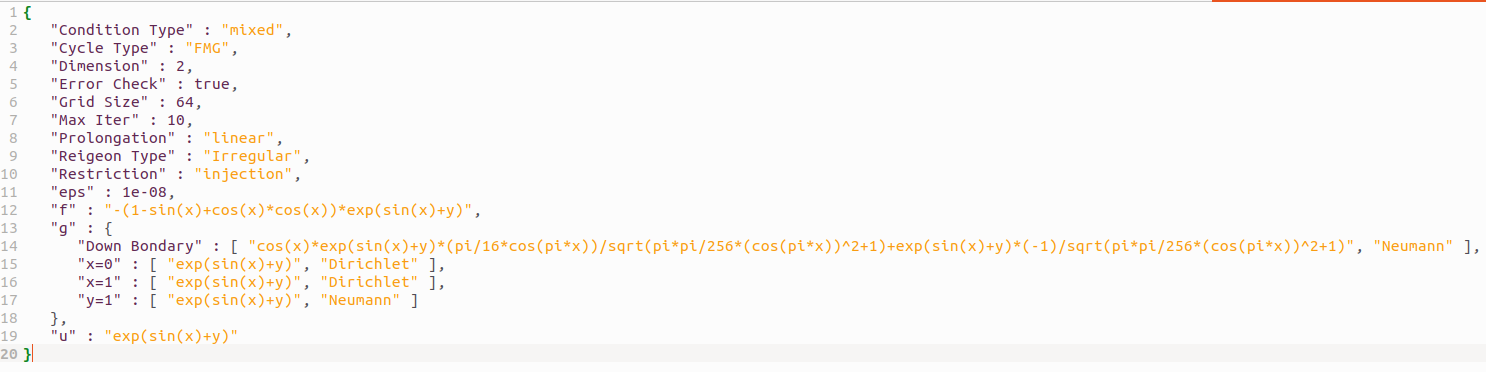
\includegraphics[width=0.88\textwidth]{pic/parm.png}
\end{figure}
\end{frame}

\begin{frame}{用户接口}
\begin{figure}[H]
\centering
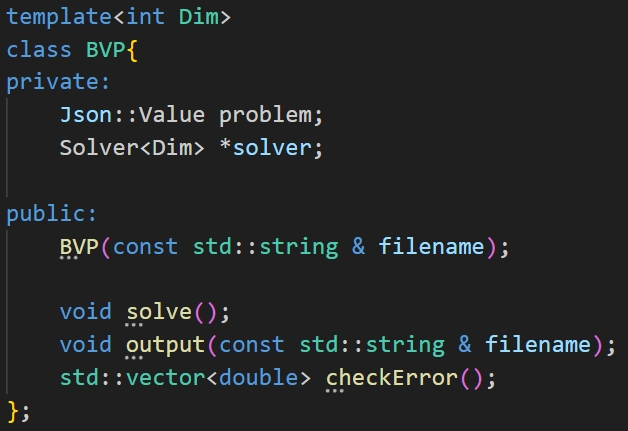
\includegraphics[width=0.6\textwidth]{pic/userPlug.png}
\end{figure}
\end{frame}

\begin{frame}{求解器类}
\begin{figure}[H]
\centering
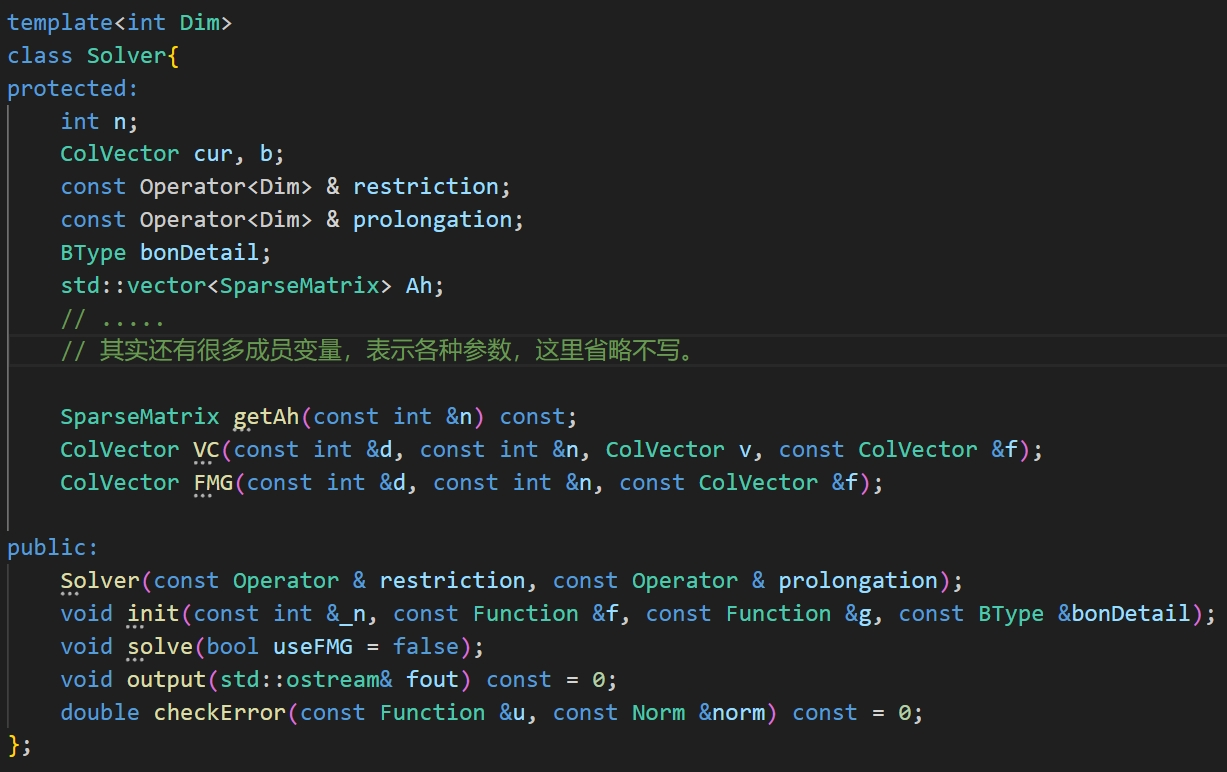
\includegraphics[width=0.95\textwidth]{pic/solver.png}
\end{figure}
\end{frame}

\begin{frame}{抽象操作类}

这是一个抽象操作类,它支持一个括号运算。
\begin{figure}[H]
\centering
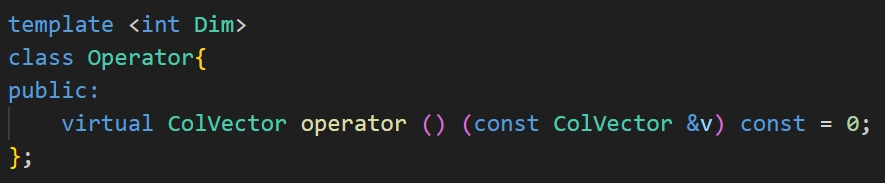
\includegraphics[width=0.95\textwidth]{pic/operator.png}
\end{figure}

\pause
它的派生类可以是插值算子,也可以是限制算子。
\begin{figure}[H]
\centering
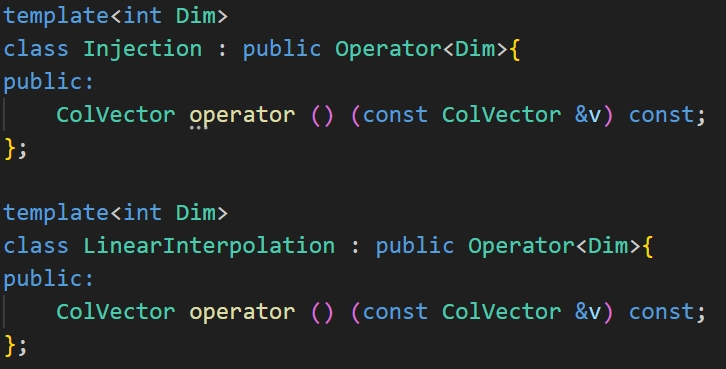
\includegraphics[width=0.75\textwidth]{pic/suboperator.png}
\end{figure}

\end{frame}

\begin{frame}{稀疏矩阵}
  一个好的多重网格求解器应该具有$O(N)$的复杂度,其中$N$是格点的数量。如果使用稠密矩阵,那么$A^h$矩阵的存储本身就有$\Theta(N^2)$的复杂度,是非常愚蠢的。

  \vspace{1em}
  \pause
  本次作业原则上禁止使用eigen的稀疏矩阵,需要自己实现。稀疏矩阵就是以$(i,j,c)$的方式存储矩阵元素,表示$A_{ij}=c$,三元组的数量是$O(N)$的。

  \vspace{1em}
  \pause
  我们用了行压缩的存储方式,具体而言,我们将元素按行、列排好序,只存储$(j,c)$,然后用一个row\_index来记录每行的第一个元素下标。矩阵乘向量的只需做元素数量次乘法,是$O(N)$的。
\end{frame}

\section{二维规则区域多重网格的理论分析}

\begin{frame}{理论分析——基本表述}
  \small
  与讲义一样,我们以齐次Dirichlet边值问题为例给出理论分析,此时的离散方程为$A^h\mathbf{u}^h=\mathbf{f}^h$,系数矩阵$A^h\in\mathbb{R}^{n^2\times n^2}$是分块矩阵,
  \begin{equation*}
    A^h=\frac{1}{h^2}\begin{bmatrix}
      T & -I & \\
      -I & T & -I & \\
      & -I & T & -I &\\
      & & \ddots & \ddots & \ddots\\
      & & & -I & T
    \end{bmatrix},\qquad \text{其中}\;\;
    T=\begin{bmatrix}
      4 & -1 & \\
      -1 & 4 & -1 & \\
      & -1 & 4 & -1 &\\
      & & \ddots & \ddots & \ddots\\
      & & & -1 & 4
    \end{bmatrix}\in\mathbb{R}^{n\times n}.
  \end{equation*}
  
  根据讲义Theorem 7.52,我们有:
  \begin{theorem}
    \small
    式(4.4)中矩阵$A^h$的特征值与对应的特征向量为:
    \begin{equation}
      \lambda_{ij}=\lambda_i+\lambda_j,\quad \mathbf{W}_{ij}=\text{vec}(\mathbf{w}_i\mathbf{w}_j^T),\quad i,j=1,...,n-1.
    \end{equation}
    其中
    \begin{equation}
      \lambda_k=\frac{4}{h^2}\sin^2\frac{kh\pi}{2},\quad w_{k,j}=\sin(jkh\pi),\quad k,j=1,...,n-1.
    \end{equation}
  \end{theorem}
\end{frame}

\begin{frame}{理论分析——基本表述}
  \small
\begin{lemma}
  \small
  式(4.4)中矩阵$A^h$的加权Jacobi迭代矩阵为:
  \begin{equation}
    T_\omega=(1-\omega)I+\omega D^{-1}(L+U)=I-\frac{\omega h^2}{4}A.
  \end{equation}

  $T_\omega$的特征向量与$A^h$一样,对应的特征值为:
  \begin{equation}
    \lambda_{ij}(T_\omega)=1-\frac{\omega h^2}{4}\lambda_{ij}=1-\omega\sin^2\frac{ih\pi}{2}-\omega\sin^2\frac{jh\pi}{2}.
  \end{equation}
\end{lemma}

\pause
\begin{definition}
  \small
  二维full-weighting算子由下式给出。
  {\tiny\hspace{-1em}
  \begin{equation*}
  v^{2h}_{i,j}=\frac{1}{16}(v^h_{2i-1,2j-1}+v^h_{2i-1,2j+1}+v^h_{2i+1,2j-1}+v^h_{2i+1,2j+1})
  +\frac{1}{8}(v^h_{2i,2j-1}+v^h_{2i,2j+1}+v^h_{2i-1,2j}+v^h_{2i+1,2j}) + \frac{1}{4}v^h_{2i,2j}.
  \end{equation*}
  }
  其中$i,j=1,...,n$. 用$\mathbf{I}_h^{2h}$表示二维full-weighting算子。
\end{definition}

\pause
\begin{definition}
  \small
  二维线性插值算子$\mathbf{I}_{2h}^h=4(\mathbf{I}_h^{2h})^T.$
\end{definition}
\end{frame}

\begin{frame}{理论分析——TG算子的谱半径}
  \small
  \begin{definition}
    \small
    对于$i,j\in[1,\frac{n}{2})$,记$i'=n-i,j'=n-j$,我们称$\mathbf{W}_{ij},\mathbf{W}_{ij'},\mathbf{W}_{ij'},\mathbf{W}_{i'j'}$为一组\textbf{互补波}。
  \end{definition}

  \pause
  \begin{lemma}
    \small
    二维full-weighting算子在一组互补波上作用的结果为:
    \begin{subequations}
      \begin{align}
        \mathbf{I}_h^{2h} \mathbf{W}_{ij}^h=c_ic_j\mathbf{W}_{ij}^{2h},\;\;
        \mathbf{I}_h^{2h} \mathbf{W}_{ij'}^h=-c_is_j\mathbf{W}_{ij}^{2h},\;\;
        \mathbf{I}_h^{2h} \mathbf{W}_{i'j}^h=-s_ic_j\mathbf{W}_{ij}^{2h},\;\;
        \mathbf{I}_h^{2h} \mathbf{W}_{i'j'}^h=s_is_j\mathbf{W}_{ij}^{2h}.
      \end{align}
    其中$i,j\in[1,\frac{n}{2}),i'=n-i,j'=n-j$. 另外
      \begin{align}
        \mathbf{I}_h^{2h}\mathbf{W}_{i\frac{n}{2}}^h&=\mathbf{0},\quad i=1,...,n-1\\
        \mathbf{I}_h^{2h}\mathbf{W}_{\frac{n}{2}j}^h&=\mathbf{0},\quad j=1,...,n-1.
      \end{align}
    \end{subequations}
  \end{lemma}

  \pause
  \begin{lemma}
    \small
    线性插值算子在波上的作用结果为:
    \begin{equation}
      I^h_{2h} \mathbf{W}_{ij}^{2h}=c_ic_j\mathbf{W}_{ij}^h-c_is_j\mathbf{W}_{ij'}^h-s_ic_j\mathbf{W}_{i'j}^h+s_is_j\mathbf{W}_{i'j'}^h,
    \end{equation}
    其中$i,j\in[1,\frac{n}{2}),i'=n-i,j'=n-j$.
  \end{lemma}
\end{frame}

\begin{frame}{理论分析——TG算子的谱半径}
  \begin{theorem}
    \small
    $\mathcal{W}_{ij}^h=\text{span}\{\mathbf{W}_{ij},\mathbf{W}_{ij'},\mathbf{W}_{ij'},\mathbf{W}_{i'j'}\}$是Two-Grid校正算子的不变子空间。
  \end{theorem}

  \pause
  \begin{lemma}
    \small
    取$\nu_1=\nu_2=3$,有$\rho(TG)<0.1$,因此能Two-Grid校正能够快速收敛。
  \end{lemma}

  \pause
  \small
  事实上,根据定理4.2,我们有:
  \begin{equation}
    TG\begin{bmatrix}
      \mathbf{W}_{ij}^h\\
      \mathbf{W}_{ij'}^h\\
      \mathbf{W}_{i'j}^h\\
      \mathbf{W}_{i'j'}^h
    \end{bmatrix} = 
    \begin{bmatrix}
      c_{11} & c_{12} & c_{13} & c_{14}\\
      c_{21} & c_{22} & c_{23} & c_{24}\\
      c_{31} & c_{32} & c_{33} & c_{34}\\
      c_{41} & c_{42} & c_{43} & c_{44}\\
    \end{bmatrix}
    \begin{bmatrix}
      \mathbf{W}_{ij}^h\\
      \mathbf{W}_{ij'}^h\\
      \mathbf{W}_{i'j}^h\\
      \mathbf{W}_{i'j'}^h
    \end{bmatrix}
  \end{equation}

  只需对每个$i,j\in[0,\frac{n}{2})$,求出相应的$C=(c_{ij})$,计算$\rho(C)$并取最大值即可得到$\rho(TG)$。
\end{frame}

\begin{frame}{理论分析——插值与限制算子的代数性质}
\small
要想证明FMG的收敛性,除了TG的谱半径,还需要variational properties:

\begin{equation}
  I_{2h}^h=c(I_h^{2h})^T,
\end{equation}
\begin{equation}
  I_h^{2h}A^hI_{2h}^h=A^{2h}.
\end{equation}

第二条成立吗?

\vspace{1em}
\pause

不成立!
\end{frame}

\begin{frame}{理论分析——插值与限制算子的代数性质}
\small
\begin{lemma}
  \small
  在$\Omega^h$中的网格点$(i,j)$上,Laplace方程可以用九点离散表示:
  \begin{align}
    \mathcal{L} u_{ij} =& \frac{1}{3h^2}(8u_{ij}-u_{(i-1)(j-1)}-u_{(i-1)j}-u_{(i-1)(j+1)}-u_{i(j-1)}-u_{i(j+1)} \nonumber \\
    &-u_{(i+1)(j-1)}-u_{(i+1)j}-u_{(i+1)(j+1)}).
  \end{align}

  由泰勒展开容易得到:$\mathcal{L} u_{ij}=-\Delta u(x_i,y_j)+O(h^4).$
\end{lemma}

我们设$B^h$为采用九点离散格式时的系数矩阵,有:
\begin{equation}
  B^h=\frac{1}{h^2}\begin{bmatrix}
    K & P & \\
    P & K & P & \\
    & P & K & P &\\
    & & \ddots & \ddots & \ddots\\
    & & & P & K
  \end{bmatrix}.
\end{equation}

\begin{equation*}
  K=\begin{bmatrix}
    8 & -1 & \\
    -1 & 8 & -1 & \\
    & -1 & 8 & -1 &\\
    & & \ddots & \ddots & \ddots\\
    & & & -1 & 8
  \end{bmatrix}\in\mathbb{R}^{n\times n}, \qquad 
  P=\begin{bmatrix}
    -1 & -1 & \\
    -1 & -1 & -1 & \\
    & -1 & -1 & -1 &\\
    & & \ddots & \ddots & \ddots\\
    & & & -1 & -1
  \end{bmatrix}\in\mathbb{R}^{n\times n}
\end{equation*}
\end{frame}

\begin{frame}{理论分析——插值与限制算子的代数性质}
  \small
  \begin{lemma}
    线性插值算子与full-weighting算子关于$B^h$具有如下共轭性质:
    \begin{equation}
      \mathbf{I}_h^{2h}B^h\mathbf{I}_{2h}^h=B^{2h}.
    \end{equation}
  \end{lemma}
\end{frame}

\begin{frame}{理论分析——FMG的收敛性}
  \small

  \begin{definition}
    \small
    对于一个正定对称矩阵$A$,我们有“$A$能量模”:$||\mathbf{u}||_A:=\langle \mathbf{u},\mathbf{u} \rangle_A=\langle A\mathbf{u},\mathbf{u} \rangle$.
  \end{definition}

  \pause
  \begin{lemma}
    \small
    二维线性插值带来的误差在$B^h$能量模下,具有如下等式。
    \begin{equation}
      ||\mathbf{I}_{2h}^h\mathbf{v}^{2h}-\mathbf{I}_{2h}^h\mathbf{u}^{2h}||_{B^h}=2||\mathbf{v}^{2h}-\mathbf{u}^{2h}||_{B^{2h}}.
    \end{equation}
  \end{lemma}

  \pause
  \begin{lemma}
    \small
    假设存在常数$K>0$,使得
    \begin{equation}
      ||\mathbf{I}_{2h}^h \mathbf{u}^{2h}-\mathbf{u}^{h}||_{B^h}\leq Kh^2.
    \end{equation}
  
    那么一次FMG-Cycle的代数误差有如下估计:
    \begin{equation}
      ||\mathbf{e}^h||_{B^h}\leq Kh^2.
    \end{equation}
  \end{lemma}

  \pause
  \begin{theorem}
    \small
    对于二维齐次Dirichlet边值问题,只需要一次FMG-Cycle迭代,就能够达到$O(h^2)$精度,计算耗时$O(N)$,$N$是格点数。
  \end{theorem}
\end{frame}


\section{代数多重网格}

\begin{frame}{背景与介绍}

代数多重网格(AMG)是几何多重网格的一个自然推广,当我们发现由偏微分方程引出的离散方程组,使用多重网格具有如此优秀的表现时,自然会想,能不能将其推广到更一般的方程组,解更一般的大型稀疏矩阵。

\pause
\vspace{1em}
答案是肯定的,这就是代数多重网格。具体而言,代数多重网格对$M$矩阵具有较好的表现,$M$矩阵是满足正定对称、对角元为正数、非对角元非正的矩阵。事实上,大部分椭圆方程的离散矩阵都是$M$矩阵。

\pause
\vspace{1em}
对一个$n\times n$的矩阵$A^h$,我们不妨将$1,...,n$看作点,将$A^h$看作一个邻接矩阵,这样我们就得到了一个稀疏图,于是就有了网格结构。

\pause
\vspace{1em}
要想应用多重网格的思路,我们必须将方程限制到粗网格中,求解后返回细网格调整。但此时我们面临着严峻的问题:我们不知道网格的结构,只知道一个矩阵。我们需要一些算法来选取粗网格点$\Omega^{2h}$,并且定义限制算子$I_{h}^{2h}$与插值算子$I_{2h}^{h}$,还要给出粗网格上的矩阵$A^{2h}$。
\end{frame}

\begin{frame}{选取粗网格点}
要想从中选取粗网格点,首先给出如下定义:

\vspace{1em}
  若$i,j$满足:
  \begin{equation}
    |a_{i,j}|\geq \theta\max_{k\neq i}|a_{i,k}|
  \end{equation}

  则称$i$强依赖于$j$,也称$j$强影响$i$. 其中$\theta$是一个事先给定的阈值.

 \vspace{.5em}
  记$N_i$为所有使$a_{i,j}\neq 0$的点$j$构成的集合,称为“相邻点”集。记$S_i$为所有强影响$i$的点构成的集合,$S_i^T$为所有强依赖于$i$的点构成的集合。

\vspace{1em}
在下文中,我们记粗网格$\Omega^{2h}=C$,细网格$\Omega^h=C\cup F$,即$F$表示所有在细网格但不在粗网格中的点。我们还记$C_i=S_i\cap C,\;D_i^s=S_i\cap F,\;D_i^w=N_i\setminus S_i$.
\end{frame}

\begin{frame}{选取粗网格点}
\small
我们希望用一种\textbf{启发式的方法}来选取粗网格点,具体地,我们希望:
\begin{enumerate}[(1)]
  \item $\forall i\in F$,对于$j\in S_i$,或$j\in C_i$,或$j$强依赖于$C_i$中某点;
  \item $C$中的点尽可能多,但需要保持:$\forall i\in C$,没有$j\in C$使得$i$强依赖于$j$。
\end{enumerate}

\pause
\vspace{1em}
当然,我们只是希望上述性质尽可能得到满足,为此,William L. Briggs的书上给出了\textbf{“染色算法”},如下:
\begin{enumerate}[1]
  \item $C,F\gets \varnothing$, $\lambda_i\gets |S_i^T|$.
  \item 选取$i\in\Omega^h\setminus(C\cup F)$,使$\lambda_i$最大.
  \item $C\gets C\cup\{i\}$, $F\gets F\cup (S_i^T\setminus C)$.
  \item $\forall j\in S_i^T,\;\forall k\in S_j\setminus(C\cup F)$, 令$\lambda_k\gets \lambda_k+1$.
  \item 若$C\cup F=\Omega^h$,结束,否则返回第2步.
\end{enumerate}

\pause
\vspace{1em}
注意到上述过程需要维护一个$\lambda_i$数组,支持增加、删除、求最大下标三种操作,我们期望单次操作的复杂度不超过$O(\log n)$,因此我们使用\textbf{二叉搜索树}。当然,使用线段树、平衡树也是可以的,不过因为可以提前建树,所以平衡操作是不必要的。
\end{frame}

\begin{frame}{构建插值算子}
\tiny
对于$\mathbf{e}\in\Omega^{2h}$,插值算子具有如下格式:
\begin{equation}
  (I_{2h}^h \mathbf{e})_i=\left\{
    \begin{array}{ll}
      e_i & \text{若 }i\in C,\\
      \sum_{j\in C_i}\omega_{ij}e_j & \text{若 }i\in F.
    \end{array}
  \right.
\end{equation}

\pause
在粗网格中,我们求解的方程是$A^{2h}\mathbf{e}=\mathbf{f}$,其中$\mathbf{f}$是光滑化(即若干次G-S迭代)后的残差,通常比较小,因此
\begin{equation*}
  a_{ii}e_i\approx -\sum_{j\in N_i} a_{ij}e_j.
\end{equation*}

\pause
将$N_i$展开成三类,得
\begin{equation}
  a_{ii}e_i\approx -\sum_{j\in C_i} a_{ij}e_j -\sum_{j\in D^s_i} a_{ij}e_j -\sum_{j\in D^w_i} a_{ij}e_j.
\end{equation}

\pause
对于$j\in D^w_i$,将$e_j$近似为$e_i$,得
\begin{equation}
  \left(a_{ii}+\sum_{j\in D^w_i} a_{ij}\right)e_i\approx -\sum_{j\in C_i} a_{ij}e_j -\sum_{j\in D^s_i} a_{ij}e_j.
\end{equation}

\pause
对于$e_j\in D_i^s$,将其近似为
\begin{equation}
  e_j\approx \frac{\sum_{k\in C_i} a_{jk}e_k}{\sum_{k\in C_i} a_{jk}}.
\end{equation}

\pause
将(6.5)代入(6.4),得
\begin{equation}
  \omega_{ij}=-\frac{a_{ij}+\sum\limits_{m\in D_i^s}\left(\frac{a_{im}a_{mj}}{\sum\limits_{k\in C_i} a_{mk}}\right)}{a_{ii}+\sum\limits_{n\in D_i^w} a_{in}}
\end{equation}

\end{frame}

\begin{frame}{构建限制算子与粗网格矩阵$A^{2h}$}

事实上,有了插值算子,我们可以直接由对称性和Garlerkin条件构建$I_{h}^{2h}$与$A^{2h}$,如下:
\begin{equation}
  I_{h}^{2h}:=(I_{2h}^{h})^T
\end{equation}
\begin{equation}
  A^{2h}:=I_{h}^{2h}A^hI_{2h}^{h}
\end{equation}

\vspace{1em}
这样variational properties总是自动满足。

\end{frame}

\begin{frame}{构建Cycle}

代数多重网格的Cycle与几何多重是一样的,只不过使用的$A^h,I_h^{2h},I_{2h}^h$都是事先构建好的。

\end{frame}


\begin{frame}
    \frametitle{谢谢}
    \centering
    \Large Thaks for your attention!
\end{frame}

\end{document}
